\documentclass[dvipdfmx, fleqn]{jsarticle}
\input{/Users/User/Documents/University/report_template/preamble/preamble}
\title{
	パターン認識 \\
	2019-04-16授業分 レポート
	}
\author{37-196360 \quad 森田涼介}
\begin{document}
\maketitle

\section*{宿題}


点群 (2D 2000点) と正規分布の十分統計量を含む
データファイルdata.mat及びdata2.matのデータに対して,
それぞれ同時対角化を適用する。


\subsection*{結果}

まず,data.matのデータについて示す。
同時対角化前の,data.matに含まれる正規分布の十分統計量は,
\begin{align}
	& \mu_1 =
		\begin{bmatrix}
			0.53823082 \\ -3.04269717
		\end{bmatrix}
	\qquad \Sigma_1 =
		\begin{bmatrix}
			 3.34176503 & 1.33496408 \\
			 1.33496408 & 1.73462199
		\end{bmatrix} \\
	& \mu_2 =
		\begin{bmatrix}
			-0.99565419 \\ 0.48512018
		\end{bmatrix}
	\qquad \Sigma_2 =
		\begin{bmatrix}
 			3.2089801 &  -0.87806376 \\
 			-0.87806376 & 3.07417451
		\end{bmatrix}
\end{align}
であった。
これらを同時対角化すると,
その変換後の正規分布の統計量は次のようになる。
なお,ここでは簡単のため,上と同じ文字を用いた。
\begin{align}
	& \mu_1 =
		\begin{bmatrix}
			0.72903906 \\ 2.89642411
		\end{bmatrix}
	\qquad \Sigma_1 =
		\begin{bmatrix}
			1.0 & 0.0 \\
			0.0 & 1.0
		\end{bmatrix} \\
	& \mu_2 =
		\begin{bmatrix}
			0.24511607 \\ -0.92796166
		\end{bmatrix}
	\qquad \Sigma_2 =
		\begin{bmatrix}
			0.57246206 & 0 \\
			0 & 3.95701516
		\end{bmatrix}
\end{align}
また,同時対角化前後の散布図を図\ref{fig:data.mat_result}に示す。

\begin{figure}
	\begin{minipage}[b]{0.45\linewidth}
		\centering
		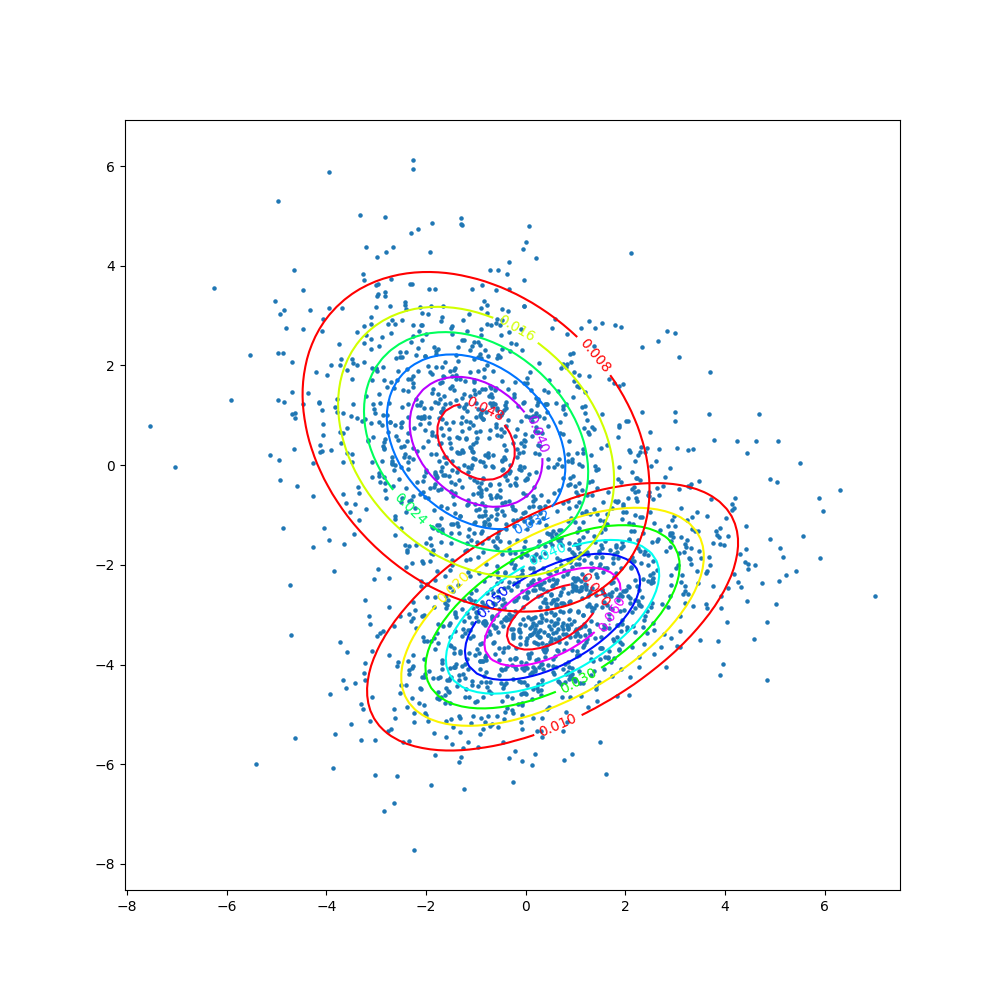
\includegraphics[clip, width=\linewidth]{../figures/scatter_before_1}
		\subcaption{同時対角化前の散布図}
		\label{fig:scatter_before_1}
	\end{minipage}
	\begin{minipage}[b]{0.45\linewidth}
		\centering
		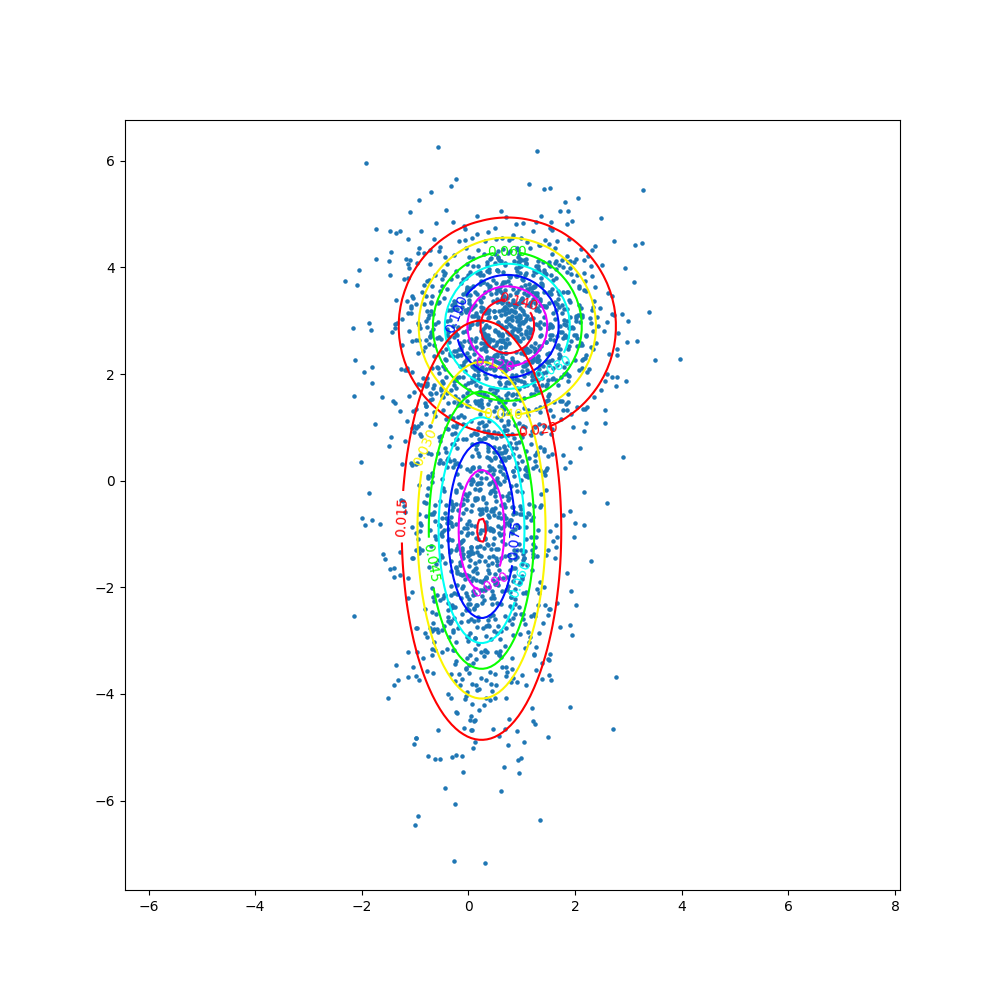
\includegraphics[clip, width=\linewidth]{../figures/scatter_after_1}
		\subcaption{同時対角化後の散布図}
		\label{fig:scatter_after_1}
	\end{minipage}
	\caption{data.matに含まれる点群についての同時対角化前後の散布図}
	\label{fig:data.mat_result}
\end{figure}


次に,data2.matのデータについて示す。
同時対角化前の,data2.matに含まれる正規分布の十分統計量は,
\begin{align}
	& \mu_1 =
		\begin{bmatrix}
			0.46886439 \\ -2.96015249
		\end{bmatrix}
	\qquad \Sigma_1 =
		\begin{bmatrix}
			3.3154755 & 1.23521877 \\
			1.23521877 & 1.69501881
		\end{bmatrix} \\
	& \mu_2 =
		\begin{bmatrix}
			-0.99565419 \\ 0.48512018
		\end{bmatrix}
	\qquad \Sigma_2 =
		\begin{bmatrix}
			0.44210079 & -0.18739151 \\
			-0.18739151 & 0.4396869
		\end{bmatrix}
\end{align}
であった。
これらを同時対角化すると,
その変換後の正規分布の統計量は次のようになる。
\begin{align}
	& \mu_1 =
		\begin{bmatrix}
			0.77239293 \\ 2.72545062
		\end{bmatrix}
	\qquad \Sigma_1 =
		\begin{bmatrix}
			1.0 & 0.0 \\
			0.0 & 1.0
		\end{bmatrix} \\
	& \mu_2 =
		\begin{bmatrix}
			0.23380354 \\ -0.9153229
		\end{bmatrix}
	\qquad \Sigma_2 =
		\begin{bmatrix}
			0.06641293 & 0 \\
			0 & 0.58577592
		\end{bmatrix}
\end{align}
また,同時対角化前後の散布図を図\ref{fig:data.mat_result}に示す。

\begin{figure}
	\begin{minipage}[b]{0.45\linewidth}
		\centering
		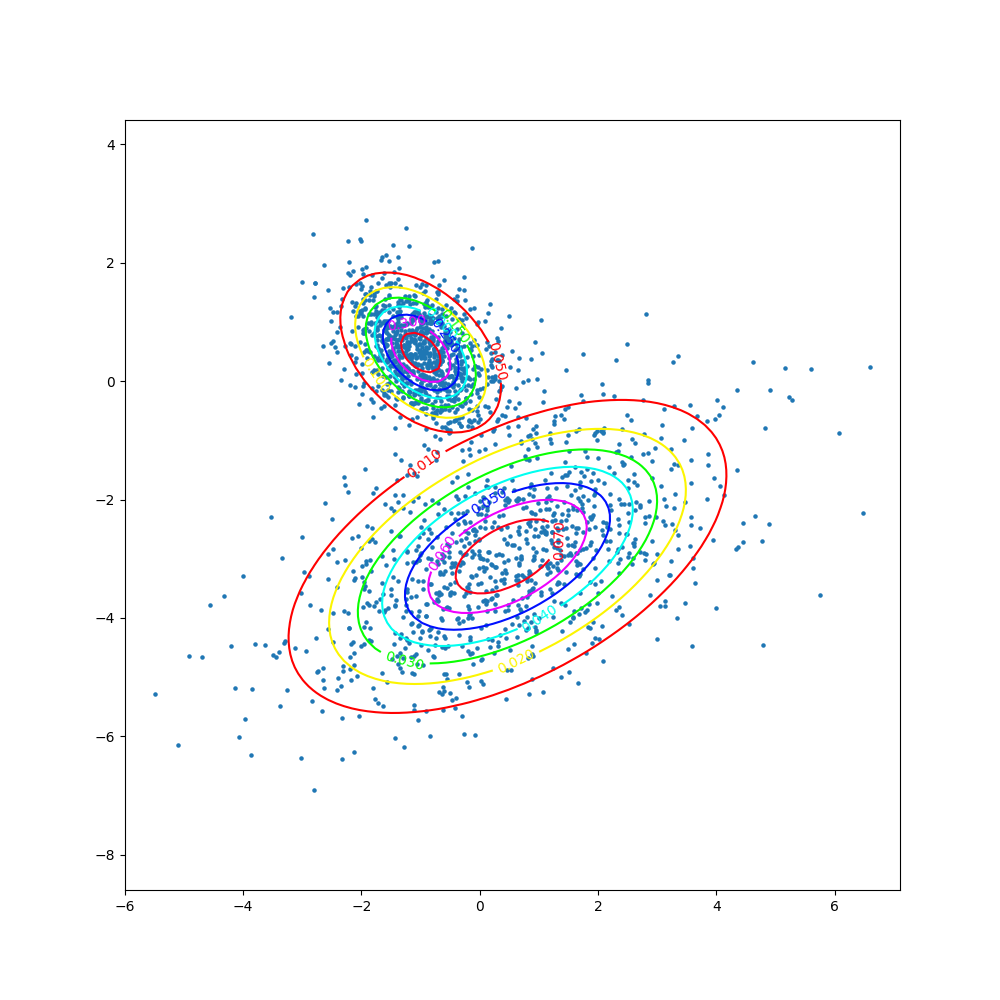
\includegraphics[clip, width=\linewidth]{../figures/scatter_before_2}
		\subcaption{同時対角化前の散布図}
		\label{fig:scatter_before_2}
	\end{minipage}
	\begin{minipage}[b]{0.45\linewidth}
		\centering
		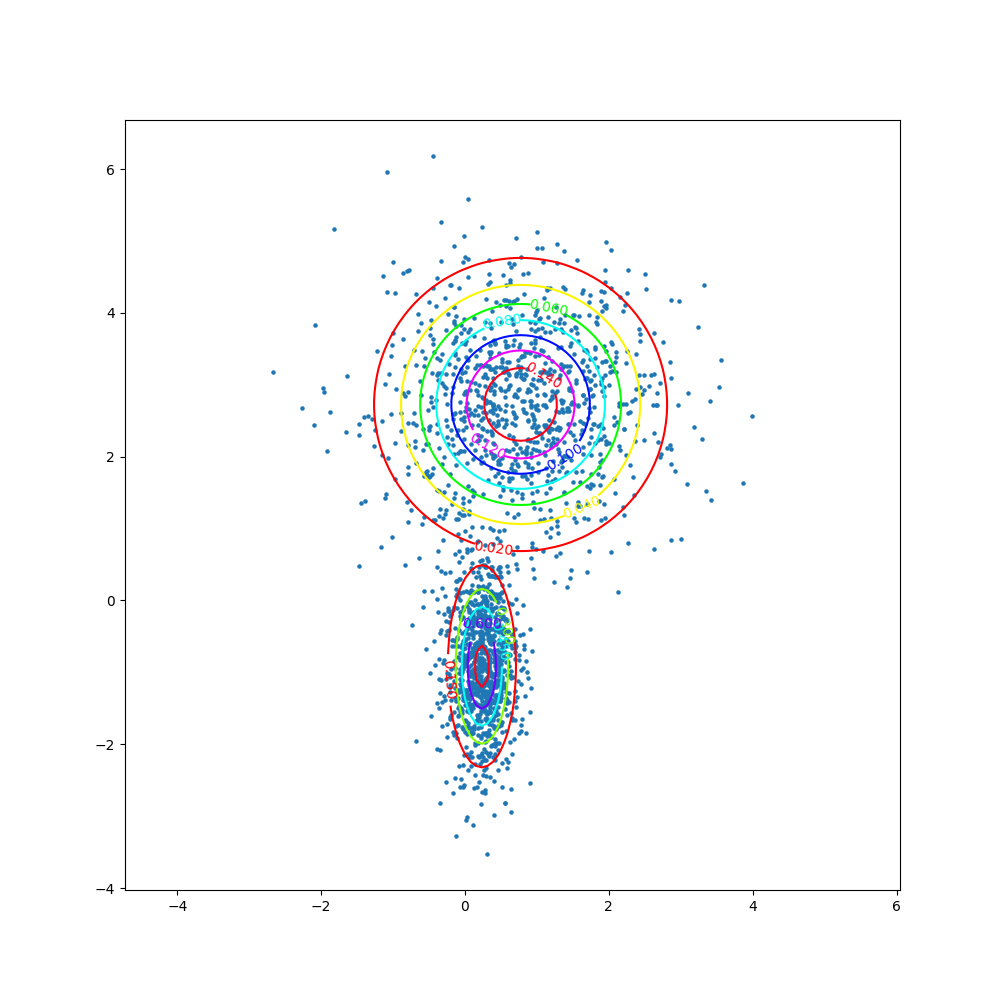
\includegraphics[clip, width=\linewidth]{../figures/scatter_after_2}
		\subcaption{同時対角化後の散布図}
		\label{fig:scatter_after_2}
	\end{minipage}
	\caption{data.matに含まれる点群についての同時対角化前後の散布図}
	\label{fig:data2.mat_result}
\end{figure}



\clearpage
\subsection*{プログラム}

プログラムは\pageref{listing:simultaneous_diagonalization}ページの
listing \ref{listing:simultaneous_diagonalization}に示した。
プログラムに含まれる関数とその簡単な説明を以下に示す。

\begin{itemize}
	\item load \\
		scipy.io.loadmatを用いて.matファイルから点群データとその正規分布の十分統計量をloadする関数
	\item print\_data \\
		点群データの型,及びその正規分布の十分統計量をconsoleに出力する関数
	\item sampling\_norm\_dist \\
		plot時に等高線を出すために,正規分布からsamplingをするための関数
	\item plot\_data \\
		点群の散布図と,その正規分布の統計量から描ける等高線を描く関数
	\item simultaneos\_diagonalize \\
		点群データとその正規分布の十分統計量に対して同時対角化を行う関数
	\item main
		実行用の関数。data\_pathという変数でdata.matを読むかdata2.matを読むかを切り替える。
\end{itemize}


なお,実行環境と用いた言語・ライブラリは以下の表\ref{tab:cp_env}に示す。

\begin{table}[H]
	\centering
	\caption{プログラムの実行環境}
	\begin{tabular}{lcl}
		OS & : & Microsoft Windows 10 Pro (64bit) \\
		CPU & : & Intel(R) Core(TM) i5-4300U \\
		RAM & : & 4.00 GB \\
		使用言語 & : & Python3.6 \\
		可視化 & : & matplotlibライブラリ
	\end{tabular}
	\label{tab:cp_env}
\end{table}

\reportlisting[listing:simultaneous_diagonalization]{simultaneous\_diagonalization.py}{../program/simultaneous_diagonalization.py}


\end{document}
